\documentclass[../didNotes.tex]{subfiles}

\begin{document}

\section{多期DID}

\begin{frame}
  \frametitle{框架}

  \begin{itemize}
    \item 多期DID是两期DID的直接扩展,从``第2期vs第1期,处理组vs控制组''扩展到``第t期vs -1期,多个处理组vs多个控制组''
    \item 两类数据:简单事件研究 $2 \times T$ 和交错设计 $G_{\#} \times T$
    \item 为了适应多期数据结构和处理机制,需要给出新的识别假设,基于识别式的估计方法和前面几乎一样
    \item 潜在因果框架 $\to$ 识别假设 $\to$ 识别式 $\to$ 估计式
    \item 两个问题:PT的检验,和TWFE的可用性
  \end{itemize}

\end{frame}

\subsection{简单事件研究}

\begin{frame}
  \frametitle{简单事件研究:定义}

  \begin{itemize}
    \item 假设有时期 $1,2, \ldots ,T$,唯一的处理发生在 $g: g\le T$ 时期,个体的接受处理标志为 $D_{i} \in \{ g,\infty \}$,个体的潜在结果是
      $$
      Y_{i,t} = \mathbb{1} (D_{i}=g) Y_{i,t}(g) + \mathbb{1} (D_{i}=\infty)Y_{i,t}(\infty)
      $$
    \item 估计目标:时期 $t$ 的ATT,共 $T-g+1$ 个待估参数
      $$
      \text{ATT}(t) \coloneqq \mathbb{E}_{\omega}[Y_{i,t}(g) - Y_{i,t}(\infty) \mid D_{i}=g]
      $$
    \item $Y_{i,t}(\infty) \mid D_{i}=g$ 是反事实,无法从数据中得到
  \end{itemize}

\end{frame}

\begin{frame}
  \frametitle{简单事件研究:识别}

  与两期DID一样,我们使用平行趋势假设(PT)来进行识别,由于有多个参数需要识别,需要多个PT假设
  \begin{assumption}[PT-ES]\label{thm:pt-es}
    潜在结果 $Y_{i,g-1}(\infty)$ 到 $Y_{i,t}(\infty)$ 在处理组和控制组里的变化趋势对于 $t:g\le t\le T$ 在平均意义上是一样的,也就是
    \begin{align*}
      &\mathbb{E}_{\omega}[Y_{i,t}(\infty) -Y_{i,g-1}(\infty) \mid D_i=g] = \\
      &\mathbb{E}_{\omega}[Y_{i,t}(\infty) - Y_{i,g-1}(\infty) \mid D_i=\infty], \; \forall t: g \le t \le T
    \end{align*}
  \end{assumption}
  假设 \ref{thm:pt-es} 允许我们来识别整个ATT序列,如果该假设只对于某些 $t$ 成立,那么可以识别出这些期的ATT
  \begin{align}
    \text{ATT}(t) & = \mathbb{E}_{\omega}[Y_{i,t}(g)-Y_{i,g-1}(\infty) \mid D_{i}=g] \nonumber \\
    & -\mathbb{E}_{\omega}[Y_{i,t}(\infty)-Y_{i,g-1}(\infty) \mid D_{i}=\infty] \nonumber \\
    & = \mathbb{E}_{\omega}[Y_{i,t}-Y_{i,g-1} \mid D_{i}=g] -
    \mathbb{E}_{\omega}[Y_{i,t}-Y_{i,g-1} \mid D_{i}=\infty] \label{eq:es-identification}
  \end{align}
\end{frame}

\begin{frame}
  \frametitle{简单事件研究:估计}

  将识别式 \eqref{eq:es-identification} 中的条件期望换成样本均值,可以写出估计式:
  $$
  \widehat{\text{ATT}}(t) = (\bar{Y}_{\omega, D=g, t}-\bar{Y}_{\omega, D=g, g-1}) -
  (\bar{Y}_{\omega, D=\infty, t}-\bar{Y}_{\omega, D=\infty, g-1})
  $$
  其无非是把两期DID估计做 $T-g+1$ 次。

  在估计出动态ATT序列后,可以对时间序列取平均,得到对时间而言``平均''的ATT
  $$
  \widehat{\text{ATT}}_{\text{avg}} \equiv \frac{1}{T-g+1} \sum_{t=g}^{T} \widehat{\text{ATT}}(t)
  $$
  从而一目了然地看出处理的平均效果。

\end{frame}

\begin{frame}
  \frametitle{简单事件研究:简单回归的偏误}
  有些实证研究者会使用如下TWFE简单回归来估计,并认为 $\hat{\beta}^{\text{twfe}}=\widehat{\text{ATT}}_{\text{avg}}$
  $$
  Y_{i,t} = \alpha_{i} + \eta_{t} + \beta^{\text{twfe}} D_{i,t} + \epsilon_{i,t}
  $$
  实际上并非如此,这个简单回归得到的系数估计是 $\widehat{\text{ATT}}_{\text{avg}}$ 减去事前趋势的均值

\end{frame}

\begin{frame}
  \frametitle{简单事件研究:简单回归的偏误}

  \begin{align*}
    \hat{\beta}^{\text{twfe}} &= (\bar{Y}_{D=1,post} - \bar{Y}_{D=1,pre}) - (\bar{Y}_{D=0,post} - \bar{Y}_{D=0,pre}) \\
    &= \frac{1}{T-g+1} \sum_{t=g}^{T} (\bar{Y}_{D=1,t}-\bar{Y}_{D=0,t}) - \frac{1}{g-1} \sum_{t=1}^{g-1}
    (\bar{Y}_{D=1,t}-\bar{Y}_{D=0,t}) \\
    &= \frac{1}{T-g+1} \sum_{t=g}^{T} \left[ (\bar{Y}_{D=1,t}-\bar{Y}_{D=0,t}) -
    (\bar{Y}_{D=1,g-1}-\bar{Y}_{D=0,g-1}) \right] \\
    &- \frac{1}{g-1} \sum_{t=1}^{g-1} \left[ (\bar{Y}_{D=1,t}-\bar{Y}_{D=0,t}) -
    (\bar{Y}_{D=1,g-1}-\bar{Y}_{D=0,g-1}) \right] \\
    &= \widehat{\text{ATT}}_{\text{avg}} - \frac{1}{g-1} \sum_{k=1}^{g-1} \hat{\tau}_{-k}
  \end{align*}

\end{frame}

\begin{frame}
  \frametitle{简单事件研究:推断}

  文献中常用的方法是用TWFE灵活回归来完成估计和推断
  \begin{align*}
    Y_{i,t} &= \alpha_i + \eta_t + \sum_{k=1}^{g-2} \beta_k \left[ \mathbb{1}(G_i=g)
    \mathbb{1}(t=k) \right] \\
    & +\sum_{s=g}^{T} \beta_s  \left[ \mathbb{1}(G_i=g) \mathbb{1}(t=s) \right] + \epsilon_{i,t} \label{eq:es-twfe}
  \end{align*}
  可以简单地证明,$\hat{\beta}_{s}=\widehat{\text{ATT}}_s$。因此,可以利用线性回归的大样本性质来构建渐进置信区间,
  或者使用bootstrap方法,\texttt{csdid} 软件包实现了这些推断方法

\end{frame}

\begin{frame}
  \frametitle{简单事件研究:用事前趋势检验PT}

  多期DID的识别依赖于(事后)PT假设 \ref{thm:pt-es},因此需要检查这一假设的可靠性。通行办法是用事前趋势估计
  \begin{align*}
    \tau_{-k} & \coloneqq \mathbb{E}[Y_{i,t=g-1-k}(\infty)-Y_{i,t=g-1}(\infty) \mid D_i = g] \\
    &-\mathbb{E}[Y_{i,t=g-1-k}(\infty)-Y_{i,t=g-1}(\infty) \mid D_i = \infty] \\
    & = \mathbb{E}[Y_{i,t=g-1-k}-Y_{i,t=g-1} \mid D_i = g] \\
    &-\mathbb{E}[Y_{i,t=g-1-k}-Y_{i,t=g-1} \mid D_i = \infty] \\
    &\leftarrow \hat{\beta}_{-k}, 0 < k < g-1
  \end{align*}
  来为PT假设提供信息,若每一期事前趋势通过t检验,那么认为PT假设成立。\textcolor{red}{最近的文献指出了这一方法的问题。}

\end{frame}

\begin{frame}
  \frametitle{``检验''PT}

  \begin{itemize}
    \item 本质问题:无法得知事后潜在结果,因此PT不可检验,事前趋势估计只是为其提供(成立或不成立的)信息
    \item 基于当期无法观测因素的处理选择机制 \parencite{ghanem2025} 使得事前趋势提供的信息无效
    \item 对事前趋势做t检验的功效较低,无法提供足够信息,需要做敏感性分析 \parencite{roth2022a,rambachan2023}
  \end{itemize}

\end{frame}

\begin{frame}
  \frametitle{``检验''PT:处理的选择机制问题}

  \textcite{ghanem2025} 证明了当处理的选择机制是当期无法观测因素的函数时,除非未处理结果满足某种鞅条件,否则无论事前趋势的形状如何,事后
  一定无法满足PT。这使我们担心:若存在这种选择机制,那么事前趋势检验将无法为PT提供有效信息。

  \vspace{1em}

  作者进一步证明,存在上述选择机制时,用平行趋势假设识别出来的ATT会具有误差
  \begin{align*}
    \Delta_{\text{post}} & = \Delta_{\text{post}}^{\text{sel}} + \Delta_{\text{post}}^{\text{mtg}}
    \\
    & = \mathbb{E}[\zeta_{i 2} \mid D_{i}=1] - \mathbb{E}[\zeta_{i 2} \mid D_{i}=0]                   \\
    & + (\rho_{2}-1) \left(\mathbb{E}[Y_{i 1} \mid D_{i}=1] - \mathbb{E}[Y_{i 1} \mid D_{i}=0]\right)
  \end{align*}
  其中,$\rho_{2}$ 满足 $\mathbb{E}[\dot{Y}_{i 2}(0) \mid \alpha_{i}, \epsilon_{i 1}]=\rho_{2} \dot{Y}_{i 1}$。
  误差分为两部分,第一部分是两组之间第二期随机冲击项的均值之差,若处理与第二期的随机冲击的实现值相关,那么第一部分将不为0;第二部分
  是鞅条件偏离程度 $\rho_{2}-1$ 和两组结果的事前差异,如果鞅条件偏离程度很远,即使检验出的事前差异很小,DID识别的偏差也是很大的。

\end{frame}

\begin{frame}
  \frametitle{``检验''PT:检验功效问题}

  \textcite{roth2022}:即使存在事后趋势,事前趋势检验会很容易通过,从而无法为PT的违反提供足够信息。

  \begin{figure}[htbp]
    \begin{center}
      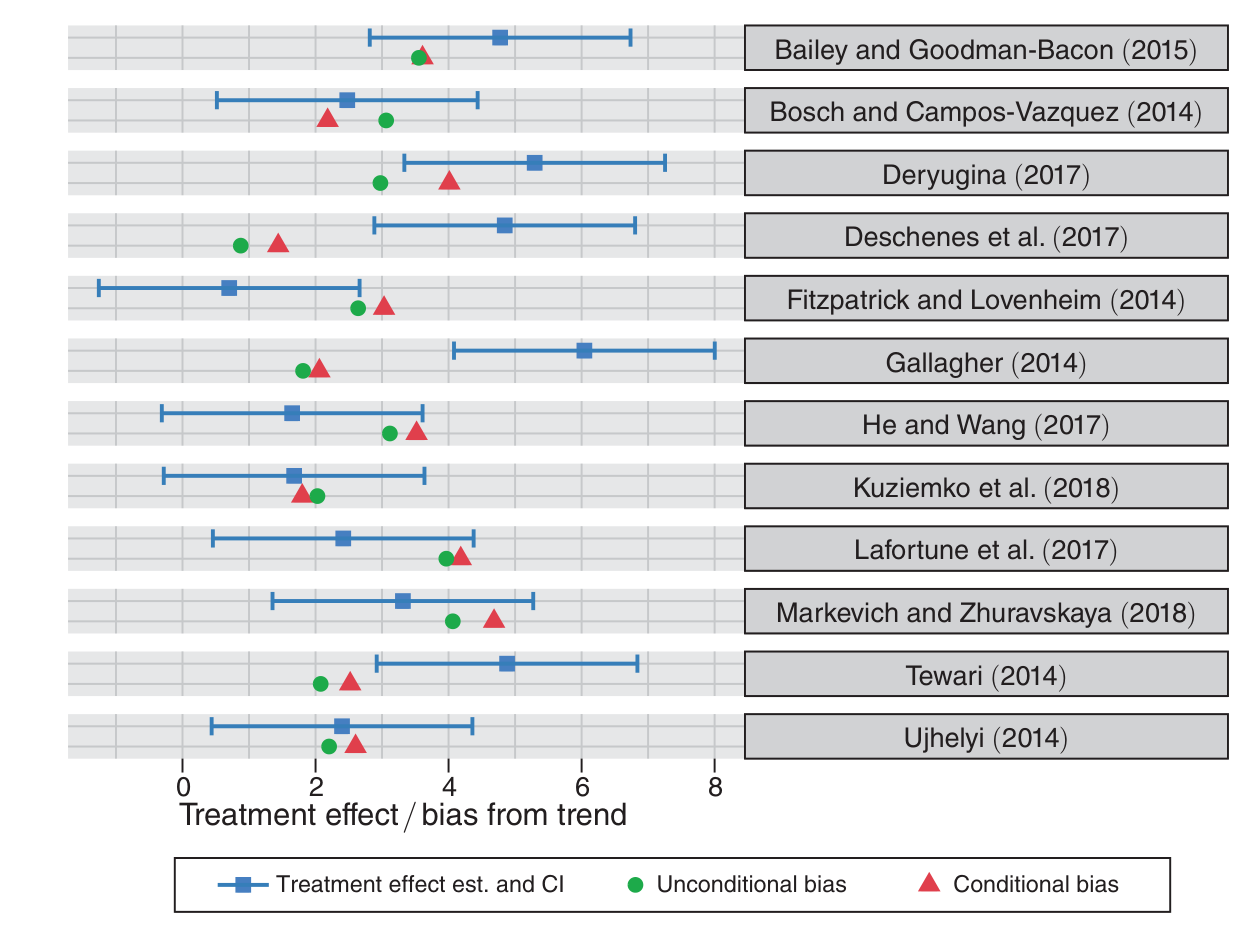
\includegraphics[width=0.6\textwidth]{./assets/PT_caution.png}
    \end{center}
    \caption{PT违反情形下DID估计量的偏差}
    \label{pic:PT_bias}
  \end{figure}

  Roth假设了一个线性违反PT的DGP,手动设定其偏离系数以使得在80\%(事前检验的功效)的情况下能够检验出事前趋势,
  并观察此时DID估计量的偏差和犯第一类错误的概率
\end{frame}

\begin{frame}
  \frametitle{``检验''PT:检验功效问题}

  当PT的违反足够大,以至于能够使得事前趋势检验在80\%的情况下检验出非平行趋势的时候,许多DID估计量的偏差甚至在绝对值上超过了估计量本身!
  如果PT的违反稍微小一点,那么事前趋势的检验效力将进一步降低,而DID估计量的偏差仍然会足以影响估计的显著性。

  \vspace{1em}
  许多情况下,平行趋势的违反没有大到足以被我们检验出来,却仍然会影响估计量的显著性。这一问题发生的主要原因是:
  \begin{itemize}
    \item 事前趋势检验是做多个t检验,单独做t检验效力低,无法检验出那种单期来看不显著,但是多期累积起来就会形成趋势的情况
    \item 聚类计算标准误时,标准误会变大,使得事前检验不容易显著
    \item 小样本下存在多重假设检验问题
  \end{itemize}

\end{frame}

\begin{frame}
  \frametitle{``检验''PT:敏感性分析}

  基于 \textcite{roth2022},\textcite{rambachan2023} 提出对PT可能被违反的情形进行敏感性分析。例如,假设
  $$
  \Delta^{\text{RM}}(M) = \{ \delta: \forall t \ge 0,\left\vert \delta_{t+1}-\delta_{t} \right\vert \le M \cdot
  \max_{s<0} \left\vert \delta_{s+1}-\delta_{s} \right\vert  \}
  $$
  在这个约束中,事后趋势偏离不会超过事前趋势偏离最大值的 $M$ 倍。\textcite{rambachan2023} 的理论贡献是推导了在类似平行趋势被
  有限度地违反地情况下,如何构造置信区间做推断。他们用这一方法对文献进行了敏感性分析,如图 \ref{pic:PT_sensitivity} 所示

\end{frame}

\begin{frame}
  \frametitle{``检验''PT:敏感性分析}

  \begin{figure}[htbp]
    \begin{center}
      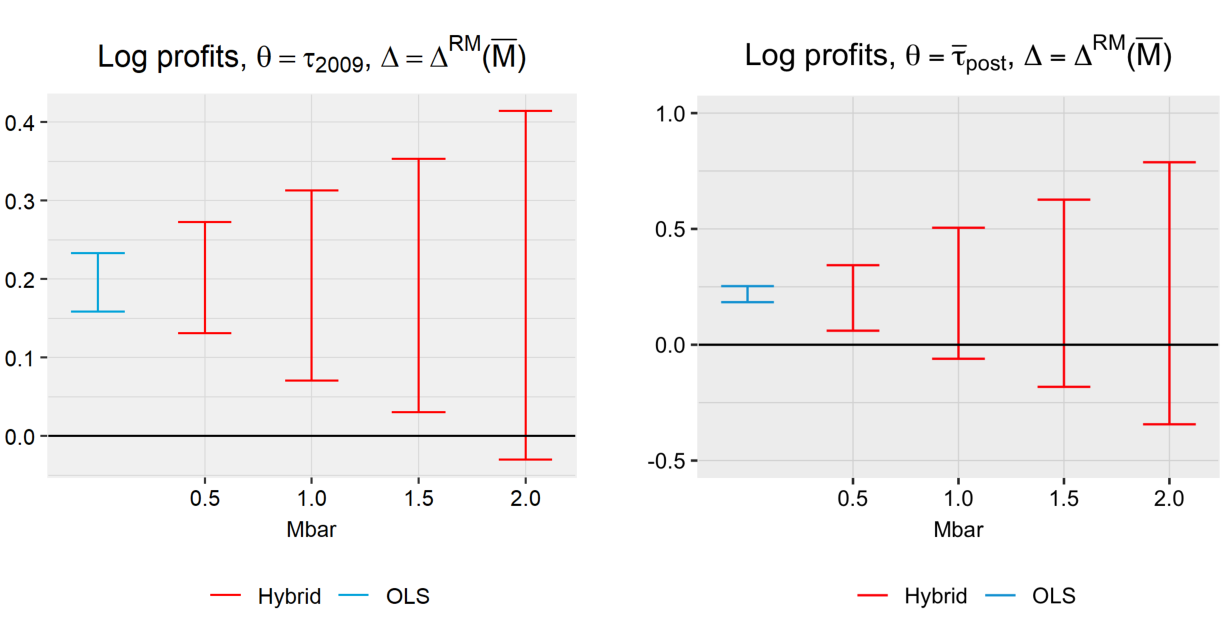
\includegraphics[width=0.8\textwidth]{./assets/PT_sensitivity.png}
    \end{center}
    \caption{对Benzarti and Carloni (2019) 的敏感性分析}
    \label{pic:PT_sensitivity}
  \end{figure}

  这里的问题在于,我们不知道 $M=2$ 是不是一个有意义的benchmark,不知道是太大还是太小,缺乏一个比较的框架。
\end{frame}

\subsection{交错DID}

\begin{frame}
  \frametitle{交错DID:定义}

  交错处理指的是不同个体在不同时间受到处理,形成不同的处理``队列''(cohort)。
  直觉上,``交错处理''将涉及\( 2 \times 2 \) 处理--对照比较。
  假设每个个体最多只会接受一次处理,且处理不会被取消,用处理开始的日期来索引潜在结果,记为 \( g: Y_{i,t}(g) \);
  对于永不接受处理的个体,我们用 \( Y_{i,t}=Y_{i,t}(\infty) \) 来表示。因此,潜在结果可以写作
  \[
    Y_{i,t} = \sum_{g \in \mathcal{G}} Y_{i,t}(g) \mathbf{1}(G_{i}=g)
  .\]
  其中 \( \mathcal{G} \) 表示所有处理时间点的集合。举例来说,假设有四期、两个处理和三个个体的数据,
  且处理分别发生在第二期和第三期,那么数据结构为
  \begin{align*}
    Y_{1,1}(\infty),Y_{1,2}(\infty),Y_{1,3}(\infty),Y_{1,4}(\infty) \\
    Y_{2,1}(2), Y_{2,2}(2), Y_{2,3}(2), Y_{2,4}(2)                  \\
    Y_{3,1}(3), Y_{3,2}(3), Y_{3,3}(3), Y_{3,4}(3)
  \end{align*}

\end{frame}

\begin{frame}
  \frametitle{交错DID:估计目标}

  在交错 DID 设计中,每一个处理队列都有自己的处理效应参数序列。称之为队列--时间平均处理效应(group-time ATT)
  \[
    \text{ATT}(g,t) \coloneqq \mathbb{E}_{\omega}[Y_{i,t}(g)-Y_{i,t}(\infty) \mid G_i = g], \forall t \ge g
  .\]
  其中 \( Y_{i,t}(\infty) \mid G_i=g \) 是反事实结果,无法从数据中直接得到。需要更加精细的PT假设来识别这一估计目标。

  \vspace{1em}
  另外,注意到group-time ATT实际上在截面和时间序列上形成了分布,可以进行处理效应的异质性分析,也可以加总得到整体性的结果。

\end{frame}

\begin{frame}
  \frametitle{交错DID:识别假设}

  在交错 DID 设计中,需要选择哪些个体作为对照组。可以选择:从未接受处理的个体(never-treated),
  以及尚未接受处理的个体(not-yet-treated,。所做的PT假设将取决于选择的对照组

  \begin{assumption}[基于从未接受处理个体的 PT,NEV]\label{thm:pt-nev}
    对于所有最终会接受处理的组 \( g \) 和处理后时期 \( t \ge g \),有
    \begin{align*}
      &\mathbb{E}_{\omega}[Y_{i,t}(\infty)-Y_{i,t-1}(\infty) \mid G_i=g] = \\
      &\mathbb{E}_{\omega}[Y_{i,t}(\infty)-Y_{i,t-1}(\infty) \mid G_i=\infty]
    \end{align*}
  \end{assumption}

  \begin{assumption}[基于尚未接受处理个体的 PT,NYT]\label{thm:pt-not-yet}
    对于所有最终会接受处理的组 \( g \),尚未接受处理的组 \( g' \),以及处理后时期
    \( t: g \le t < g' \),有
    \begin{align*}
      &\mathbb{E}_{\omega}[Y_{i,t}(\infty)-Y_{i,t-1}(\infty) \mid G_i=g] = \\
      &\mathbb{E}_{\omega}[Y_{i,t}(\infty)-Y_{i,t-1}(\infty) \mid G_i=g']
    \end{align*}
  \end{assumption}

\end{frame}

\begin{frame}
  \frametitle{交错DID:识别假设(con't)}

  一些文献还使用更严格的PT假设——要求PT在所有时期和所有组中都成立——来构造更精确和有效的估计量
  \begin{assumption}[所有时期与所有组的 PT,ALL]\label{thm:pt-all}
    对于任意两个组 \( g,g' \) 和时期 \( t \),有
    \begin{align*}
      &\mathbb{E}_{\omega}[Y_{i,t}(\infty)-Y_{i,t-1}(\infty) \mid G_i=g] = \\
      &\mathbb{E}_{\omega}[Y_{i,t}(\infty)-Y_{i,t-1}(\infty) \mid G_i=g']
    \end{align*}
  \end{assumption}

\end{frame}

\begin{frame}
  \frametitle{交错DID:识别(NEV)}

  把假设 \ref{thm:pt-nev} 代入 \( \text{ATT}(g,t) \) 得到
  \[
    \text{ATT}(g,t) = \mathbb{E}_{\omega}[Y_{i,t}-Y_{i,g-1} \mid G_i=g] -
    \mathbb{E}_{\omega}[Y_{i,t}-Y_{i,g-1} \mid G_i=\infty]
  .\]
  由此可以识别。结合前面的例子,这个估计量可以构造为
  \begin{align*}
    \widehat{\text{ATT}}(2,2) & =[Y_{2,2}-Y_{2,1}] - [Y_{1,2}-Y_{1,1}] \\
    \widehat{\text{ATT}}(2,3) & =[Y_{2,3}-Y_{2,1}] - [Y_{1,3}-Y_{1,1}] \\
    \widehat{\text{ATT}}(3,3) & =[Y_{3,3}-Y_{3,1}] - [Y_{1,3}-Y_{1,1}]
    .
  \end{align*}
\end{frame}

\begin{frame}
  \frametitle{交错DID:识别(NYT)}

  利用假设 \ref{thm:pt-not-yet} 可以识别 ATT:
  \[
    \text{ATT}(g,t) = \mathbb{E}_{\omega}[Y_{i,t}-Y_{i,g-1} \mid G_i=g] -
    \mathbb{E}_{\omega}[Y_{i,t}-Y_{i,g-1} \mid G_i > \max \{g,t\} ]
  .\]
  结合前面的例子,该估计量可以构造为
  \begin{align*}
    \widehat{\text{ATT}}(2,2) & = [Y_{2,2}-Y_{2,1}] - \frac{1}{2} [Y_{1,2}-Y_{1,1} +
    Y_{3,2}-Y_{3,1}].
  \end{align*}
  其他估计量与NEV情形相同。

\end{frame}

\begin{frame}
  \frametitle{交错DID:识别假设的选择}

  面对三类识别假设,我们该选哪一种?
  \begin{enumerate}
    \item ALL(假设 \ref{thm:pt-all}):因为使用了更多的数据,可以得到更加精确的估计量;但是这一假设本身比较严格,如果某些队列-时间下PT不满足,那么估计量是有偏的
    \item 在NEV假设下(假设 \ref{thm:pt-nev}):只将从未接受处理的个体作为对照组,这一做法简单直观,也避免了``forbidden
      comparisons''的麻烦,估计量可以直接用一个回归得到;但如果这些个体是由于某些特质而选择没有接受处理,那么PT可能会不满足,而且有的时候这部分个体可能比较少,会使得估计效率降低
    \item NYT(假设 \ref{thm:pt-not-yet})是一个中庸之选,相比于ALL假设要求更放松,相比于NEV假设可以使用更多信息,但是无法通过回归直接估计,需要采用``前向工程''方法进行估计和推断
  \end{enumerate}

\end{frame}

\begin{frame}
  \frametitle{交错DID:估计}

  \begin{itemize}
    \item 不带协变量情况,无非是把 $\text{ATT}(g,t)$ 的识别式中的期望换成样本均值,注意对照组的选择
    \item 带协变量的情况,对每个 $\text{ATT}(g,t)$ 采用DR方法进行估计即可
  \end{itemize}

  问题:什么情形下,TWFE估计量是可用的(也就是等价于``前向工程''思想所构造出来的估计量)?

\end{frame}

\begin{frame}
  \frametitle{交错DID:加总}

  \begin{itemize}
    \item 所有处理个体与时间的平均效应:\( \text{ATT}_{\text{agg}}
      \coloneqq \sum_{g,t} w_{\omega, g,t} \text{ATT}(g,t) \)
    \item 事件发生后 \( e \) 期的平均效应:\(
        \text{ATT}_{\text{es}}(e) \coloneqq \sum_{g < \infty} w^{\text{es}}_{\omega, g, e}
      \text{ATT}(g,g+e)  \)
    \item 特定队列的平均效应:\( \text{ATT}_{\text{es}}(g) \coloneqq
      \sum_{0 \le e \le T-g} w^{\text{es}}_{\omega, g, e} \text{ATT}(g,g+e)  \)
  \end{itemize}

  其中,权重由研究者手动来选取,和为1。
\end{frame}

\begin{frame}
  \frametitle{TWFE的可用性}

  表 \ref{tab:TWFE} 展示了最近文献中对不同DID设置下TWFE适用性的讨论

  \begin{table}[ht]
    \caption{TWFE可用性比较}\label{tab:TWFE}
    \centering
    {\scriptsize
      \begin{tabularx}{\linewidth}{@{} p{3.2cm} *{2}{C} L p{3.2cm} @{}}
        \toprule
        DID设计 & 简单回归 & 灵活回归 & 文献 \\
        \midrule
        两期 & $\checkmark$ & -- & -- \\
        两期带协变量 & $\times$ & -- & \textcite{caetano2024} \\
        多期 & $\checkmark$ (minus pre-effect) & $\checkmark$ & -- \\
        多期带协变量 & $\times$ & $\times$ & \textcite{callaway2021} \\
        交错-NEV & $\times$ & $\checkmark$ (IW) & \textcite{sun2021} \\
        交错-NYT & $\times$ & $\times$ & -- \\
        交错-ALL & $\times$ & $\checkmark$ (ETWFE) & \textcite{wooldridge2021} \\
        交错带协变量 & $\times$ & $\times$ & \textcite{callaway2021} \\
        \bottomrule
      \end{tabularx}
    }
  \end{table}

\end{frame}

\begin{frame}
  \frametitle{TWFE的可用性-2}

  \textbf{任何带有协变量的情形}。这一问题在前面的部分已经说明。一旦带有协变量,TWFE形式下的系数估计将会是所有的CATT以非凸权重进行加总,其因果含义
  不清晰。因此,文献中建议使用``前向工程方法'',也就是首先使用RA、IPW或者DR方法估计出CATT,再进行加总得到ATT。

  \vspace{1em}

  \textbf{简单事件研究情形}。这一问题在前面的部分已经说明。在简单事件研究情形下,采用灵活回归可以正确识别并估计 $\text{ATT}(t)$,而采用
  简单回归,得到的是所有 $\text{ATT}(t)$ 的均值减去事前``效应''的均值,因此需要做调整。

\end{frame}

\begin{frame}
  \frametitle{TWFE的可用性-3}

  \textbf{交错情形}。在交错情形下,采用简单回归得到的估计量 $\hat{\beta}^{\text{twfe}}$ 是有问题的,
  简单回归的设定本质上也是不同队列的处理组和其控制组做差得到的ATT的加权平均,然而其中隐含了一些
  ``forbidden comparisons'',也就是包含了``将已经受到处理的队列作为控制组''的比较。这一行为的问题在于,它会给某些队列--时期的ATT赋予
  负的权重。考虑一个3期3队列的设定,这三个队列分别在第一期、第二期和第无穷期接受处理。此时,可以把简单回归的第二期数据减掉第一期数据,得到
  $$
  \Delta Y_{i,2} = \Delta \eta_{2} + \beta^{\text{twfe}} \Delta D_{i,2} + \Delta \epsilon_{i,2}
  $$
  对于第一期和无穷期接受处理的组而言,$\Delta D_{i,2}=0$,对于第二期接受处理的组而言,$\Delta D_{i,t}=1$,因此上式是一个二值回归,得到的
  估计值就是difference-in-mean:

\end{frame}

\begin{frame}
  \frametitle{TWFE的可用性-4}

  \textbf{交错情形}
  \begin{align*}
    \beta^{\text{twfe}} &= \mathbb{E}[\Delta Y_{i,2} \mid \Delta D_{i,2}=1] - \mathbb{E}[\Delta Y_{i,2} \mid
    \Delta D_{i,2}=0] \\
    &= \left(\mathbb{E}[\Delta Y_{i,2} \mid G_{i}=2] - \mathbb{E}[\Delta Y_{i,2} \mid G_{i}=\infty]\right)(1-w_{1}) \\
    &+\left(\mathbb{E}[\Delta Y_{i,2} \mid G_{i}=2] - \mathbb{E}[\Delta Y_{i,2} \mid G_{i}=1]\right)w_{1} \\
    &= \cdots \\
    &= \text{ATT}(2,2)(1-w_{1}) + \left( \text{ATT}(2,2)-[\text{ATT}(1,2)-\text{ATT}(1,1)] \right) w_{1} \\
    &= \text{ATT}(2,2)+w_{1} \text{ATT}(1,1) - w_{1} \text{ATT}(1,2)
  \end{align*}
  结果上来看,$\beta^{\text{twfe}}$ 包含了在时期二将第二组和第一组(已经接受处理)进行比较,
  从而导致最后的结果出现了带有负权重的 $\text{ATT}(g,t)$ 加总,这甚至可能导致TWFE估计结果和实际的加总结果 $\text{ATT}_{\text{avg}}$
  符号相反!
  在交错情形下,\textcite{sun2021} 证明了,即使是采用灵活回归,每一个系数所对应的估计目标依然存在上述问题,因此,灵活回归也不可用。

\end{frame}

\begin{frame}
  \frametitle{TWFE的可用性-5}

  \textbf{交错情形}。文献中对TWFE进行了一系列拓展,使其在一定的PT假设下,能够估计得到和``前向工程''下一样的ATT估计量。
  比如说,\textcite{sun2021} 所提出的interaction--weighted估计量
  $$
  Y_{i,t} = \alpha_{i} + \eta_{t} + \sum_{g \neq \infty} \sum_{e \neq -1} \beta_{g,e}^{\text{IW}} \mathbb{1} (G_{i}=g)
  \mathbb{1}(G_{i}+e=t) + \epsilon_{i,t}
  $$
  可以在NEV假设下一致地估计出各个 $\text{ATT}(g,t)$,再进行加总;而 \textcite{wooldridge2021} 所提出的ETWFE估计量
  $$
  Y_{i,t} = \alpha_{i} + \eta_{t} + \sum_{g \neq \infty} \sum_{s = g}^{T} \beta_{g,t}^{\text{E}} \mathbb{1} (G_{i}=g)
  \mathbb{1}(s=t) + \epsilon_{i,t}
  $$
  可以在ALL假设下一致地估计出各个 $\text{ATT}(g,t)$,再进行加总。

\end{frame}

\begin{frame}
  \frametitle{总结}

  这篇综述建议实证研究者在使用DID进行研究时,应当按照以下步骤进行:
  \begin{enumerate}
    \item 根据数据结构与处理类型确定待估参数,比如说,明确要估计的是 $\text{ATT(g,t)}$
    \item 明确识别假设(哪些组之间存在PT)
    \item 选择合适估计方法进行估计(一般而言,就是用IPW或者DR),对异质性(队列,时间)的估计结果进行分析,加总得到整体的估计结果
    \item 讨论不确定性的来源,进行推断(design, sampling or model based)
    \item 对PT做敏感性分析
  \end{enumerate}

\end{frame}

\end{document}
